\subsection{DECOVALEX unsaturated test case}
DECOVALEX is an international code comparison project for the verification of thermo-hydro-mechanical (THM) and thermo-hydro-chemical (THC) numerical simulators \cite{BirEtAl:2008}.

\subsubsection*{Definition}
The original DECOVALEX-THM benchmark definition is a 2-D problem \cite{BirEtAl:2008}. For the comparison of different HM swelling models, we consider a simplified case representing a horizontal cross-section through the 2-D domain. Examined here is the isothermal HM consolidation problem with unsaturated flow.

\begin{figure}[!t]
\begin{center}
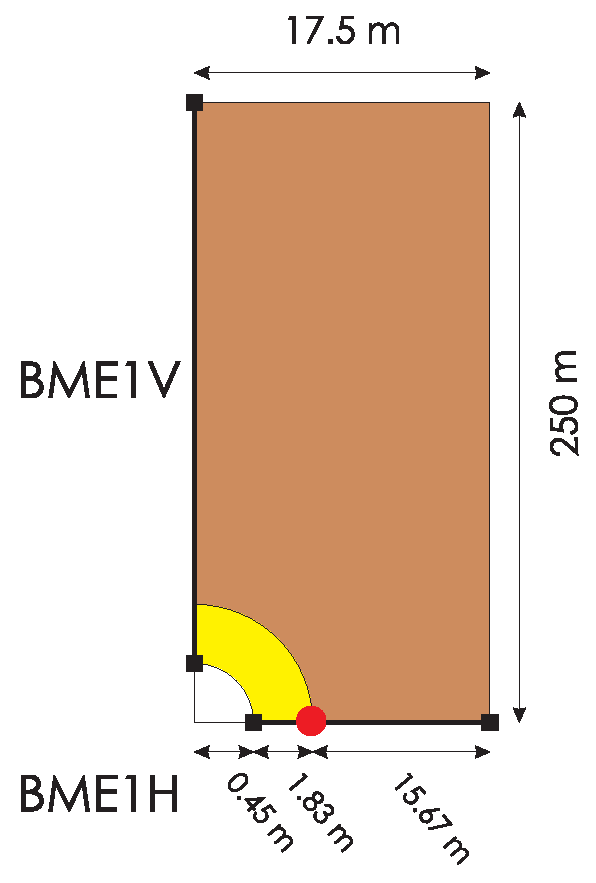
\includegraphics[width=0.3\textwidth]{chapter_14/figures/fig_14_2_15}
\end{center}
\caption{2D DECOVALEX HM definition and simplification for the benchmark exercise BME1H.}
\label{fig:thm-1D}
\end{figure}

\begin{figure}[!t]
\begin{center}
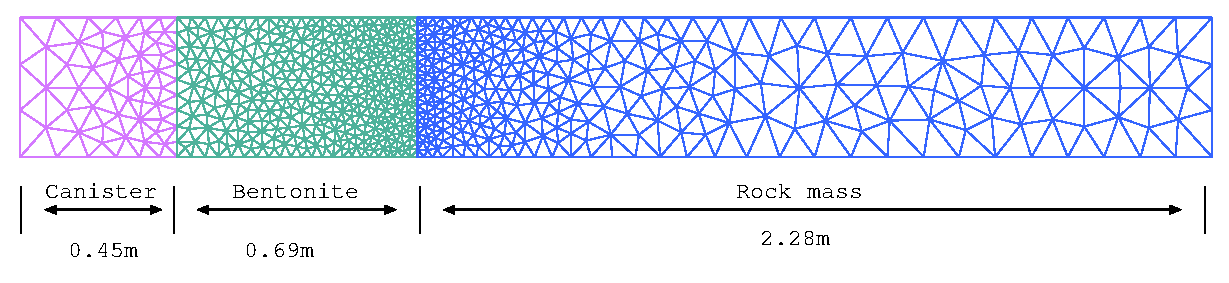
\includegraphics[width=1.0\textwidth]{chapter_14/figures/fig_14_2_16}
\end{center}
\caption{Mesh of the simplified BME1H model including canister, bentonite, and rock mass sections.}
\label{fig:thm-1Dmesh}
\end{figure}

The simplified model takes a rectangle shape. The mesh of the domain together with material types are shown in Fig. \ref{fig:thm-1Dmesh}. Fig. \ref{fig:BME1H} illustrates the definition of initial and boundary conditions for the horizontal cross-section. Observation points are set at $x=0.45\,m, \,x=1.10\,m$ to record temporal breakthrough curves. Material parameters for the rock mass and bentonite are given in Table \ref{tab:hm_rock}.

\begin{table}[!thb]
\begin{center}
\begin{tabular}{lll}
\hline
Parameter   &  Unit  & Value\\
\hline
\textit{Rock mass properties} & & \\
Density &  $kg/m3$ &  2700 \\
Young's modulus &  $GPa$ &  $35$ \\
Poisson ratio & - &  0.3 \\
Porosity & - &  0.01 \\
Saturated permeability &  $m2$  & $1.0\times10^{-17}$ \\
\\
\textit{Bentonite properties} & & \\
Density &  $kg/m3$ &  1600 \\
Young's modulus &  $MPa$ &  $317$\\
Poisson ratio & - &  0.35 \\
Saturated permeability &  $m2$  & $2.0
\times10^{-21}$ \\
\hline
\end{tabular}
\end{center}
\caption{\label{tab:hm_rock}Solid properties of different materials.}
\end{table}

\begin{figure}[!htb]
\begin{center}
%\footnotesize
\scalebox{0.8} % Change this value to rescale the drawing.
{
\begin{pspicture}(0,-1.900625)(18.579687,1.900625)
\definecolor{color7g}{rgb}{1.0,0.0,0.2}
\definecolor{color0g}{rgb}{0.4,0.4,0.4}
\definecolor{color0f}{rgb}{0.6,0.6,0.6}
\psframe[linewidth=0.04,dimen=outer,fillstyle=gradient,gradlines=2000,gradbegin=color0g,gradend=color0f,gradmidpoint=1.0](12.799687,1.0171875)(1.7796875,-1.1428125)
\psframe[linewidth=0.04,dimen=outer,fillstyle=gradient,gradlines=2000,gradbegin=color7g,gradend=color7g,gradmidpoint=1.0](3.7996874,1.0171875)(1.7596875,-1.1228125)
\psframe[linewidth=0.04,dimen=outer,fillstyle=gradient,gradlines=2000,gradbegin=blue,gradend=blue,gradmidpoint=1.0](6.4396877,1.0171875)(3.7796874,-1.1428125)
\psframe[linewidth=0.04,dimen=outer](18.539688,1.4571875)(18.519688,1.2971874)
\usefont{T1}{ptm}{m}{n}
\rput(7.403125,1.5271875){$u_y$=0, $\sigma_{xy}$=0}
\usefont{T1}{ptm}{m}{n}
\rput(7.383125,-1.6728125){$u_y$=0, $\sigma_{xy}=0$}
\usefont{T1}{ptm}{m}{n}
\rput(14,0.2471875){$u_x=0, \sigma_{xy}=0$}
\usefont{T1}{ptm}{m}{n}
\rput(13.8,-0.1){$p^l=10^6$Pa}
\usefont{T1}{ptm}{m}{n}
\rput(0.973125,0.2471875){$u_x$=0}
\usefont{T1}{ptm}{m}{n}
\rput(0.99,-0.1){$\sigma_{xy}$=0}
\usefont{T1}{ptm}{m}{n}
\rput(5.,0.24){\color{red}S0=0.65}
\usefont{T1}{ptm}{m}{n}
\rput(5.1,-0.1){\color{yellow}($p^l=-7\times10^7$Pa)}
\usefont{T1}{ptm}{m}{n}
\rput(9,-0.1728125){\color{yellow}$p^l=10^5$Pa}
\end{pspicture}
}
\end{center}
\caption{Simplified horizontal cross-section model.}
\label{fig:BME1H}
\end{figure}

The dependency of capillary pressure and relative permeability on liquid saturation for both rock and bentonite are depicted in Fig. \ref{fig:cp_cp}.

\begin{figure}[!htb]
\begin{center}
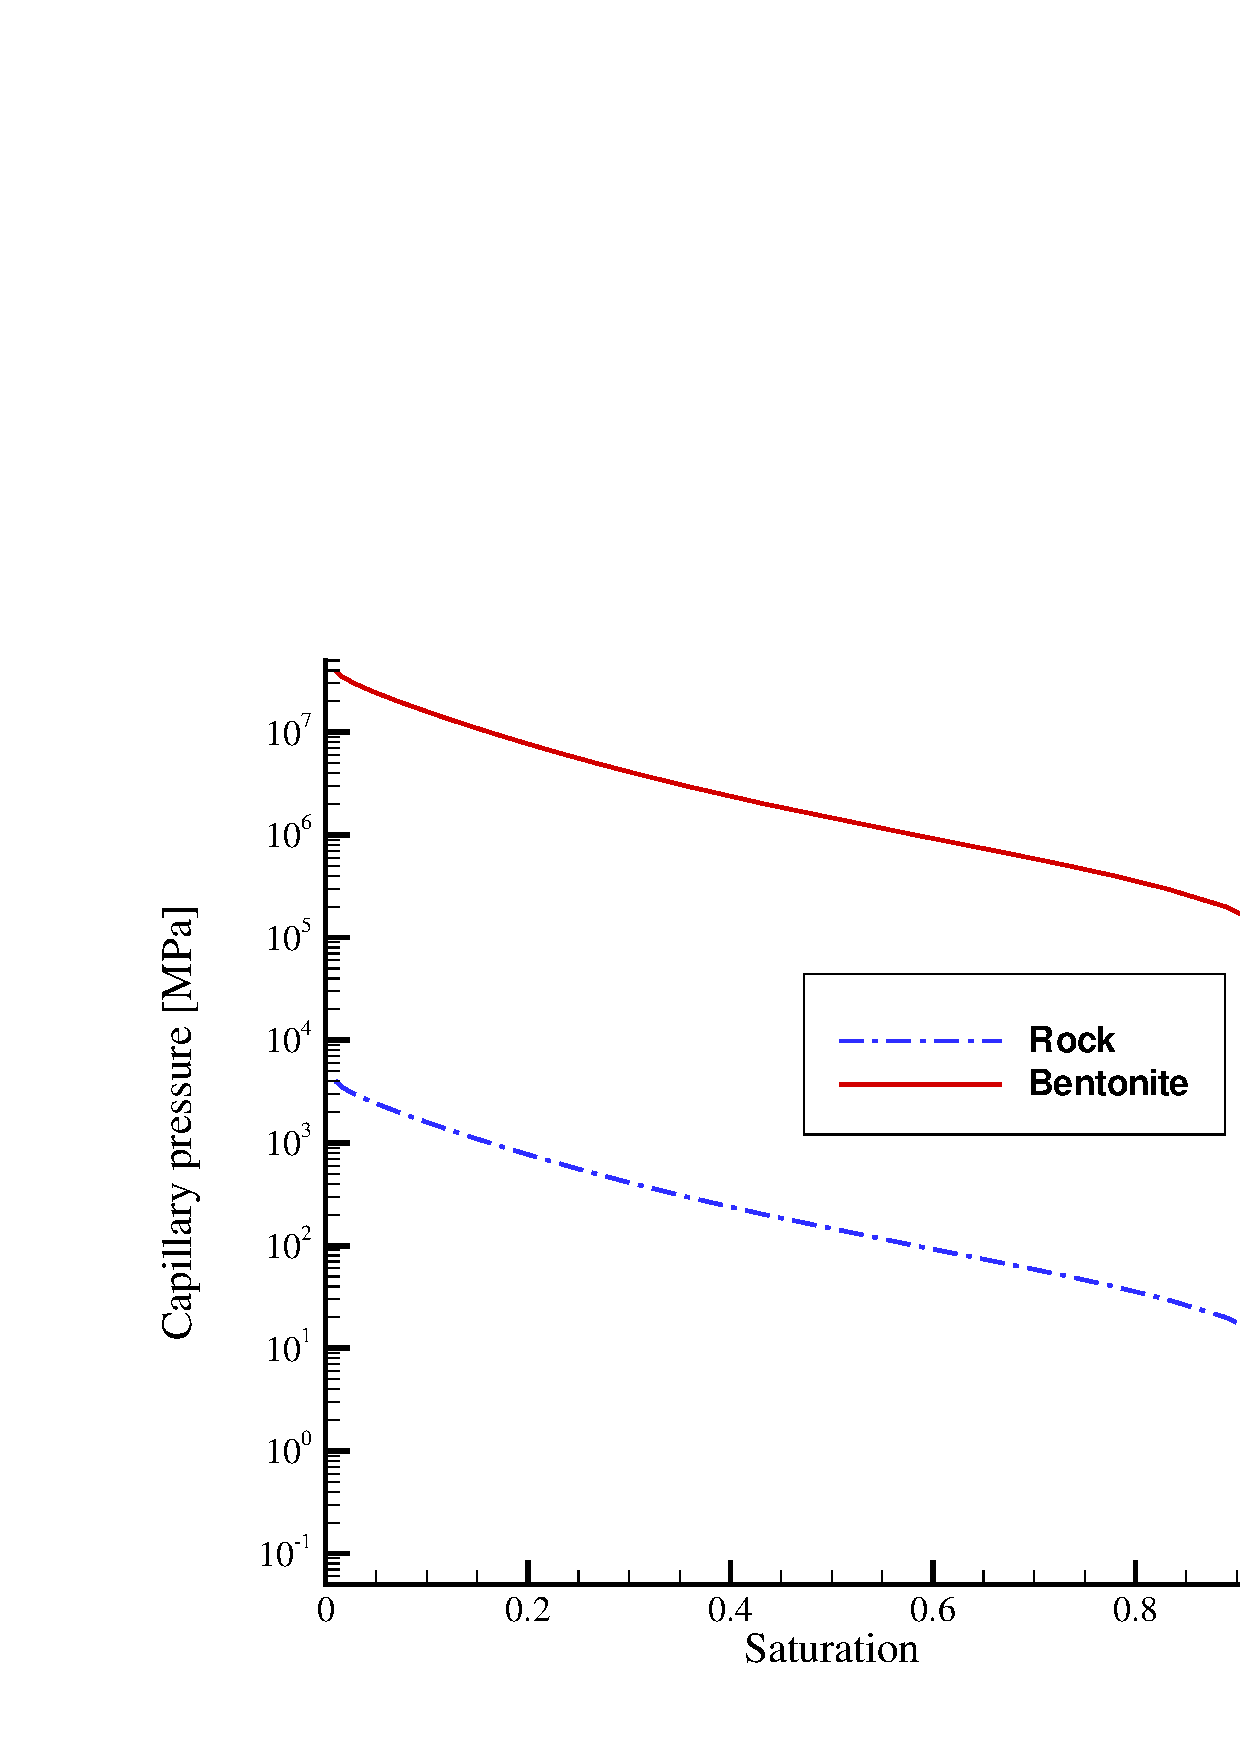
\includegraphics[width=0.49\textwidth]{chapter_14/figures/fig_14_2_18_a}
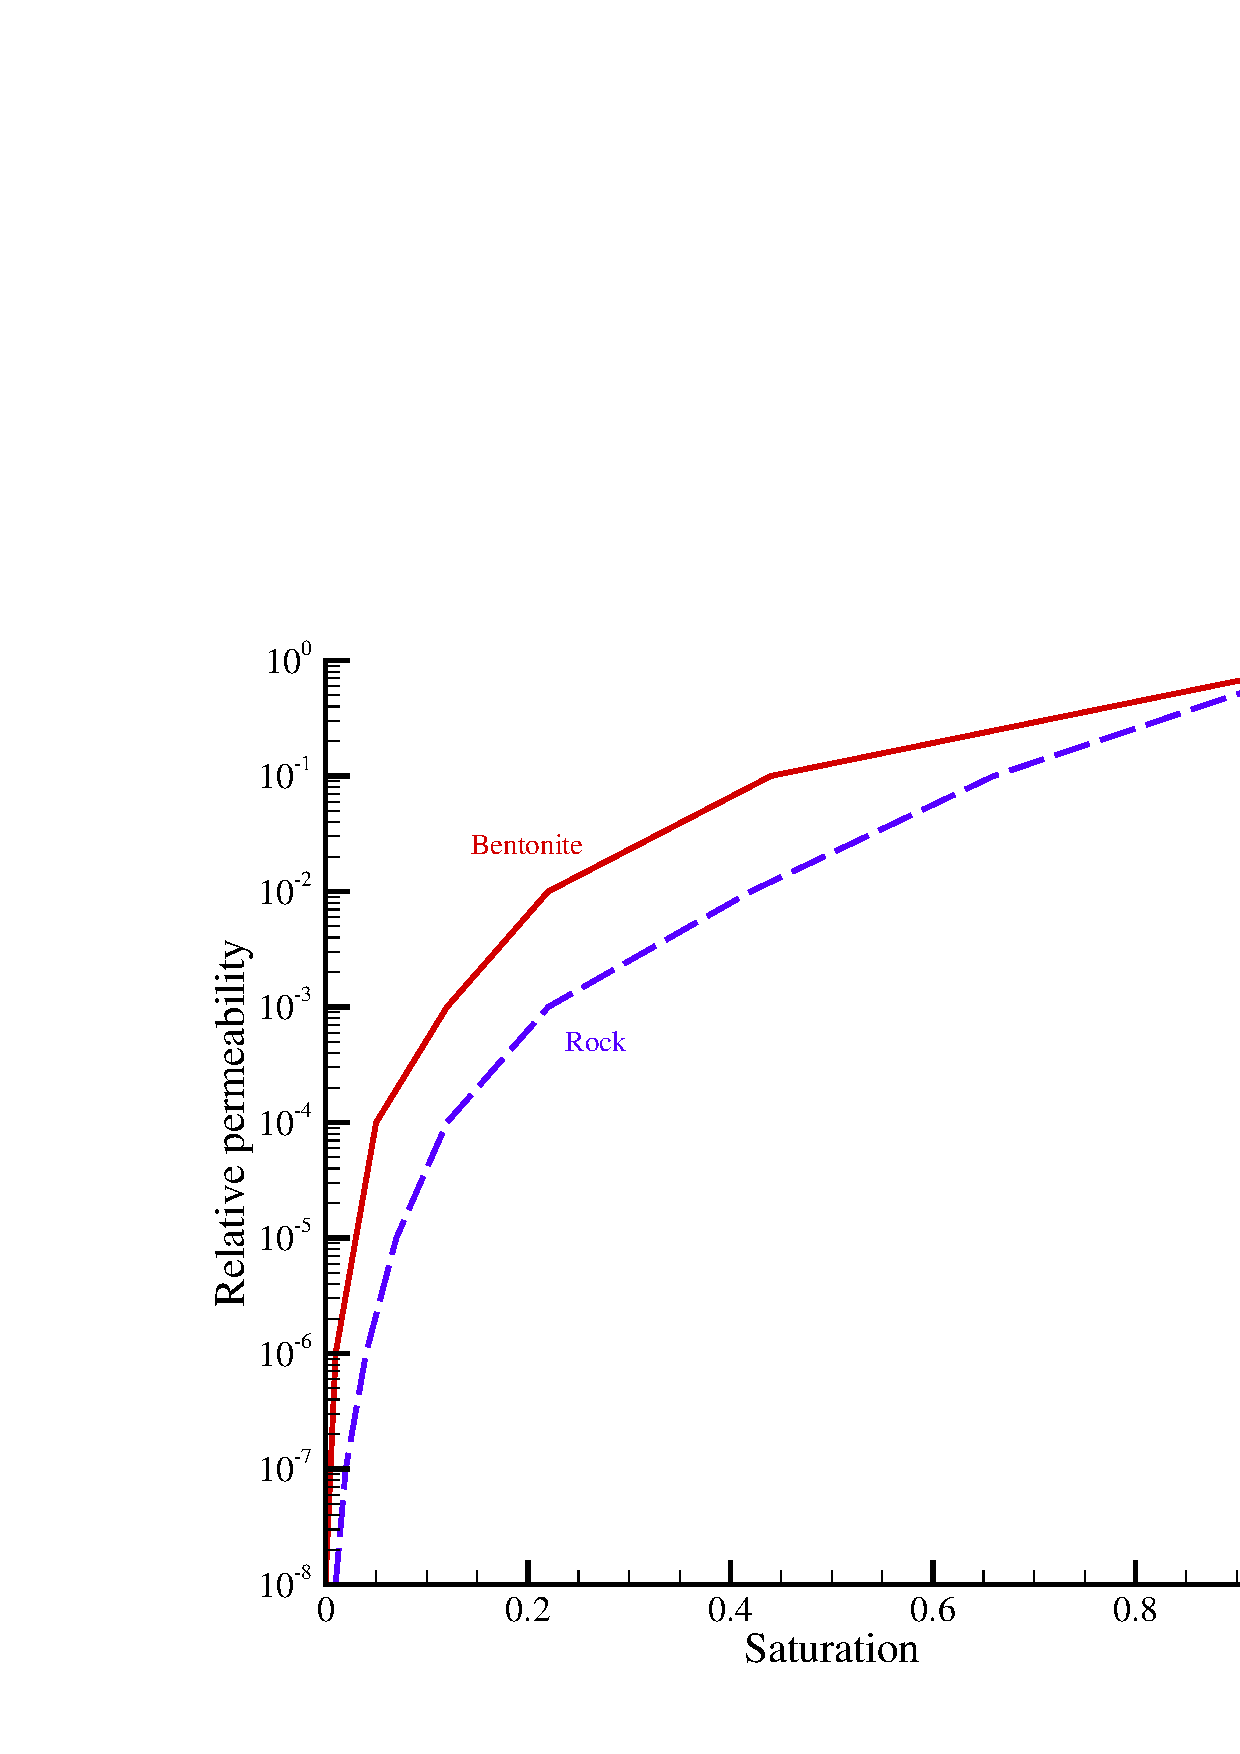
\includegraphics[width=0.49\textwidth]{chapter_14/figures/fig_14_2_18_b}
\end{center}
\caption{Capillary pressure and relative permeability functions.}
\label{fig:cp_cp}
\end{figure}

\begin{figure}[!t]
\begin{center}
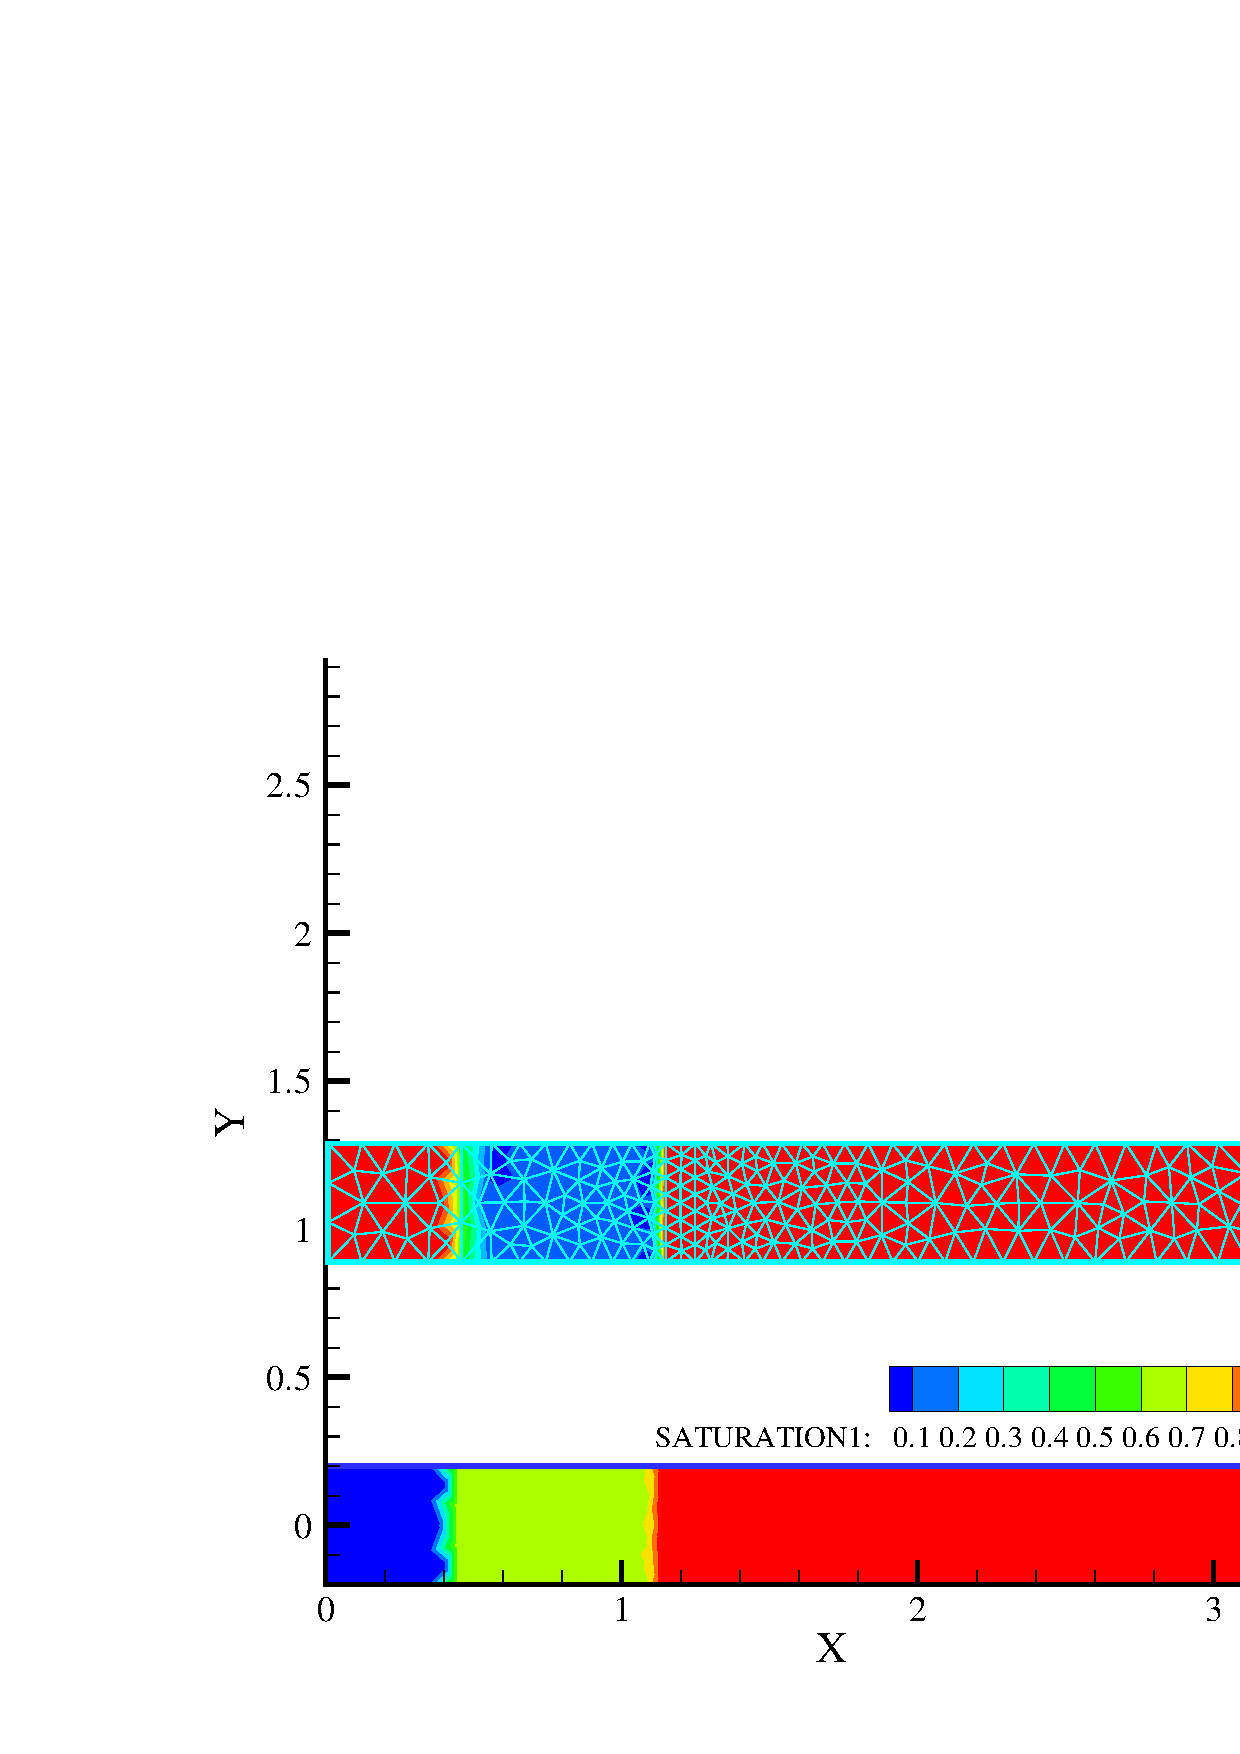
\includegraphics[width=0.7\textwidth]{chapter_14/figures/fig_14_2_19}
\end{center}
\caption{Distribution of saturation and vertical swelling stress}
\label{fig:hmswl_cont}
%\end{figure}
%\begin{figure}[!t]
\begin{center}
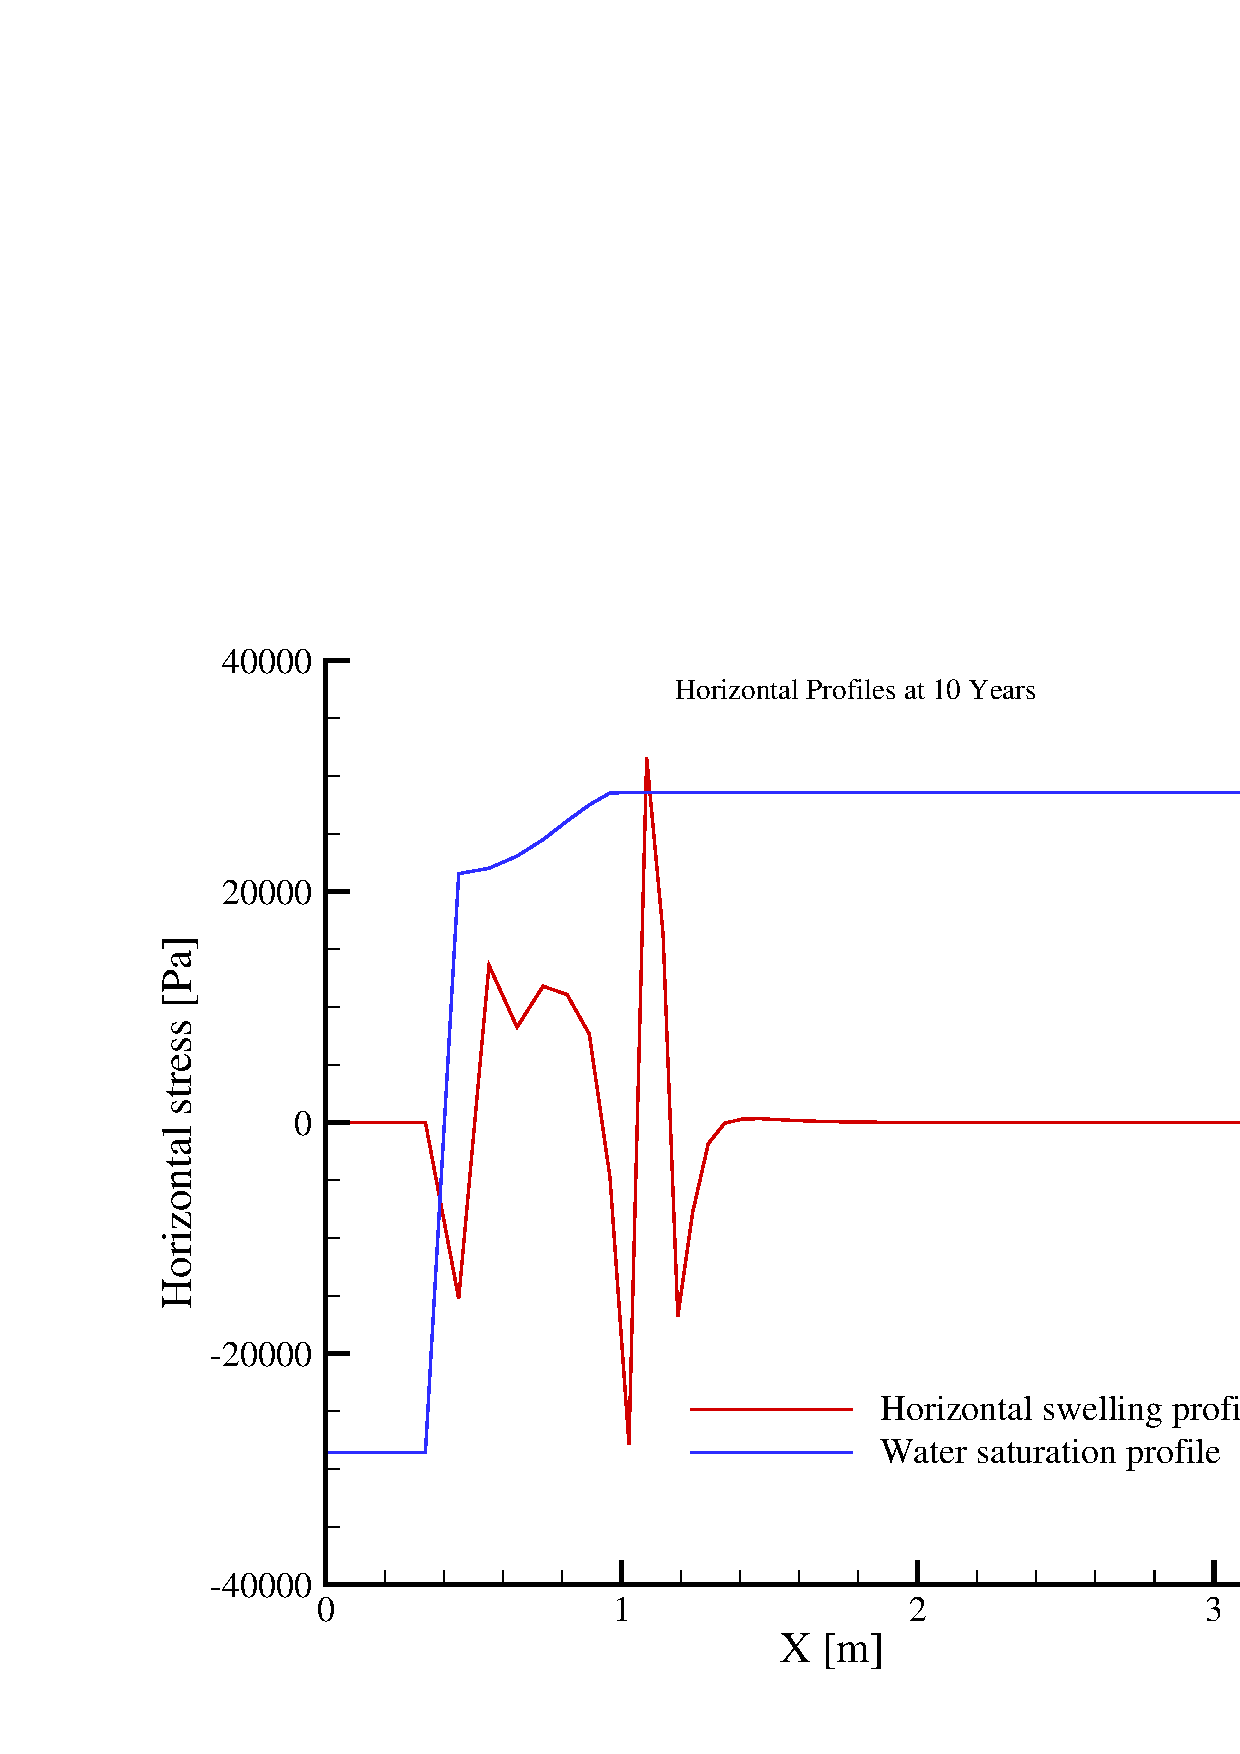
\includegraphics[width=0.49\textwidth]{chapter_14/figures/fig_14_2_20_a}
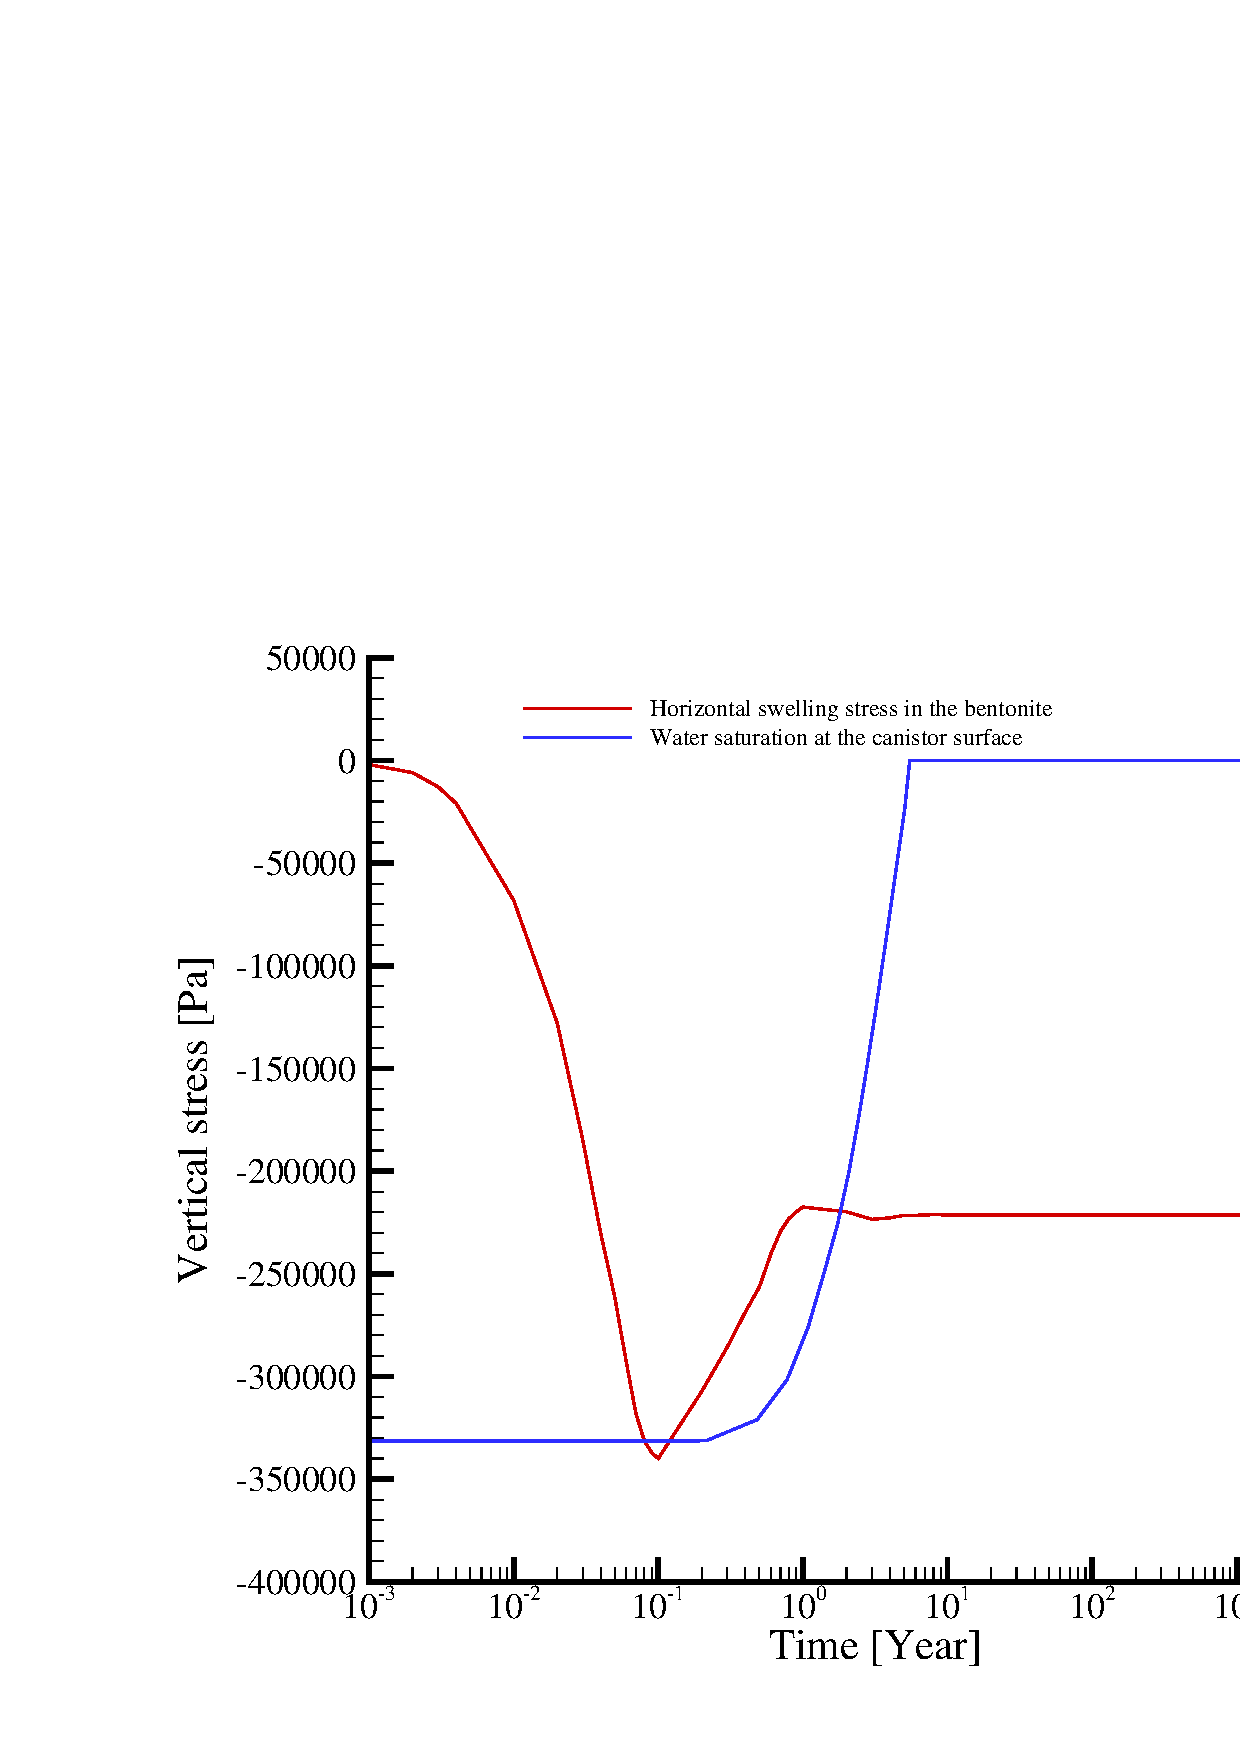
\includegraphics[width=0.49\textwidth]{chapter_14/figures/fig_14_2_20_b}
\end{center}
\caption{Horizontal profile (top) and temporal evolution at observation point (bottom) of water saturation and swelling stress}
\label{fig:deco-hm}
\end{figure}

\subsubsection*{Results}
Fig. \ref{fig:hmswl_cont} displays a contour plot of saturation and vertical swelling stress in the domain. Swelling stress in the bentonite is clearly induced by change of water saturation. Fig. \ref{fig:deco-hm} shows the simulated horizontal profiles (top) and temporal evolutions at the observation point (bottom) of water saturation and swelling stress based on the linear swelling model proposed by Rutqvist (2005) \cite{Jonny05}, which defines the increment of swelling stress to be proportional to liquid saturation increment,

\begin{equation}
\Delta \sigma ^{sw}=\beta \Delta S_w,
\end{equation}

where $\beta $ is a swelling coefficient that could be called the maximum swelling stress. As the saturation change approaches unity, swelling stress approaches $\beta $.

Fig. \ref{fig:deco-hm} shows the simulated horizontal profiles and temporal evolutions at the observation point of water saturation and swelling stress based on the linear swelling model proposed by Rutqvist (2005) \cite{Jonny05}.